\documentclass[11pt,a4paper,twoside]{article}
\usepackage[margin=2.2cm]{geometry}
\usepackage{amsmath,amssymb,amsfonts,bm}
\usepackage{graphicx}
\usepackage{booktabs,multirow,array}
\usepackage{caption,subcaption}
\usepackage{hyperref}
\usepackage{tikz}
\usetikzlibrary{positioning,arrows.meta,shapes.geometric,fit,calc,decorations.pathreplacing}
\usepackage{float}
\usepackage{enumitem}
\usepackage{fancyhdr}
\usepackage{xcolor}

\definecolor{ofdmgreen}{HTML}{2ca02c}
\definecolor{zpblue}{HTML}{1f77b4}
\definecolor{pcpred}{HTML}{d62728}

\newcommand{\E}{\mathbb{E}}
\newcommand{\CN}{\mathcal{CN}}
\newcommand{\Hest}{\hat{H}}
\newcommand{\hest}{\hat{h}}
\newcommand{\nest}{\hat{\sigma}^2}
\newcommand{\xhat}{\hat{\mathbf{x}}}
\newcommand{\F}{\mathbf{F}}
\newcommand{\B}{\mathbf{B}}
\newcommand{\G}{\mathbf{G}}
\newcommand{\I}{\mathbf{I}}
\newcommand{\y}{\mathbf{y}}

\pagestyle{fancy}
\fancyhead[LE,RO]{\thepage}
\fancyhead[RE]{OFDM vs OTFS Comparison}
\fancyhead[LO]{Technical Report}
\fancyfoot{}

\title{\Large\bfseries OFDM vs OTFS Waveform Comparison\\for High-Mobility Wireless Communications:\\[6pt]
\large A Practical Assessment with Estimated CSI,\\Noise Estimation, and 3GPP Channel Models}

\author{P.~Alevizos\thanks{Renesas Electronics. Email: bigpan27@gmail.com. Analysis, simulation, and report preparation in collaboration with Claude (Anthropic).}}
\date{April 2026 — v1.0}

\begin{document}
\maketitle
\thispagestyle{empty}

\begin{abstract}
Orthogonal Time Frequency Space (OTFS) modulation exploits the delay-Doppler domain to achieve full time-frequency diversity in doubly-selective channels. However, the majority of published OTFS evaluations rely on \emph{oversimplified assumptions}: perfect channel knowledge, oracle noise power, integer Doppler, and unlimited pilot guard zones. These idealizations mask the true performance gap between OTFS and the well-established OFDM baseline.

This report bridges this gap by implementing and comparing three complete waveform architectures under \emph{fully practical conditions}: (i)~5G NR OFDM with linear channel estimation and DMRS-based noise estimation; (ii)~ZP-OTFS with delay-Doppler impulse pilot and time-domain LMMSE equalization; and (iii)~PCP-OTFS with Zadoff-Chu pilot, GCE-BEM channel estimation, and frequency-domain equalization. All methods use estimated CSI, estimated noise power, and identical 3GPP TDL channel realizations.

Simulations across four bandwidth configurations (SCS~$\in\{15, 30, 60\}$~kHz, FFT~$\in\{256, 512\}$) reveal that the \emph{subcarrier spacing}---not the waveform---is the dominant performance factor. PCP-OTFS outperforms OFDM by 4--37$\times$ at SCS~$\leq$~15~kHz with $f_D \geq 500$~Hz, while OFDM dominates at SCS~$= 60$~kHz. The cyclic prefix design, pilot structure, and channel estimation quality are identified as the key differentiators.
\end{abstract}

\tableofcontents
\newpage

%═══════════════════════════════════════════════════════════════
\section{Introduction}
\label{sec:intro}
%═══════════════════════════════════════════════════════════════

\subsection{Motivation}

Fifth-generation (5G) and beyond wireless systems must support increasingly challenging mobility scenarios: high-speed trains at 500~km/h, vehicle-to-everything (V2X) communications, low-Earth-orbit (LEO) satellite links with Doppler shifts exceeding 40~kHz, and unmanned aerial vehicle (UAV) data links. In all these scenarios, the wireless channel is \emph{doubly selective}---varying simultaneously in both time (Doppler) and frequency (delay spread).

OFDM, the dominant waveform in 4G/5G, converts a wideband frequency-selective channel into parallel narrowband flat-fading subchannels via cyclic prefix insertion. This elegant approach breaks down at high Doppler: the channel changes within one OFDM symbol, causing inter-carrier interference (ICI) that grows with the ratio $f_D / \Delta f$, where $f_D$ is the maximum Doppler frequency and $\Delta f$ is the subcarrier spacing (SCS).

OTFS modulation \cite{hadani2017} was proposed to address this limitation by multiplexing data in the \emph{delay-Doppler} (DD) domain, where the channel is sparse and approximately time-invariant. Each DD-domain symbol spreads across the entire time-frequency plane, potentially achieving the full diversity offered by the doubly-selective channel.

\subsection{Critique of Prior Art}

The OTFS literature presents compelling theoretical advantages. However, most published evaluations employ one or more of the following oversimplifications:

\begin{enumerate}[label=(\roman*)]
    \item \textbf{Perfect CSI:} The receiver is given the exact channel impulse response, bypassing the estimation problem entirely. This is particularly problematic because, as we demonstrate, channel estimation is the \emph{primary bottleneck} for OTFS performance.
    
    \item \textbf{Known noise power:} The LMMSE/MMSE equalizer regularization term $\sigma^2$ uses the true noise variance from the simulation parameters, which is unavailable at a practical receiver.
    
    \item \textbf{Integer Doppler:} Many analyses restrict Doppler shifts to exact multiples of the DD grid resolution $\Delta\nu = 1/(NT)$, avoiding the fractional Doppler problem that causes spectral leakage across all Doppler bins via the Dirichlet kernel.
    
    \item \textbf{Unlimited pilot guard:} The DD pilot guard zone is sized to capture the full channel response, without accounting for the overhead cost. For channels with large delay-Doppler spread, this overhead can exceed 25\%.
    
    \item \textbf{Mismatched comparisons:} OFDM baselines often use suboptimal configurations (low SCS, poor channel estimation) while OTFS uses ideal settings.
\end{enumerate}

\subsection{Contributions}

This report provides a fair, systematic comparison under practical conditions:
\begin{itemize}[nosep]
    \item Complete TX/RX chain implementation for three waveform architectures (OFDM, ZP-OTFS, PCP-OTFS) with estimated CSI and estimated noise power
    \item Derivation and comparison of noise estimation methods for each waveform, including a novel decorrelated DMRS power-difference estimator for OFDM
    \item Analysis of CP/ZP design impact: ZP length sweep, Doppler bin sweep, overhead scaling
    \item Systematic evaluation across 4 bandwidth configurations, 3 channel models, 3 Doppler frequencies, and 7 SNR points
    \item Identification of the SCS as the dominant factor, not the waveform itself
\end{itemize}

%═══════════════════════════════════════════════════════════════
\section{Channel Model}
\label{sec:channel}
%═══════════════════════════════════════════════════════════════

We adopt the 3GPP Tapped Delay Line (TDL) channel model from TS~38.901. The discrete-time baseband channel at sampling rate $F_s$ is:
\begin{equation}
    y[k] = \sum_{i=0}^{L_{ch}-1} h_i[k] \, x[k - \tau_i] + w[k]
    \label{eq:channel}
\end{equation}
where $h_i[k] = \alpha_i[k]\sqrt{P_i}$ is the complex gain of the $i$-th tap at sample $k$, $\tau_i$ is the delay (in samples), $P_i$ is the average power (from the TDL profile), and $w[k] \sim \CN(0, \sigma^2)$ is additive white Gaussian noise.

The time-varying fading coefficient $\alpha_i[k]$ is generated by the Jakes sum-of-sinusoids model:
\begin{equation}
    \alpha_i[k] = \frac{1}{\sqrt{N_s}} \sum_{n=1}^{N_s} e^{j(2\pi f_D \cos(\phi_{i,n}) k T_s + \psi_{i,n})}
\end{equation}
where $N_s = 64$ sinusoids, $\phi_{i,n}$ and $\psi_{i,n}$ are uniformly distributed random phases, $f_D$ is the maximum Doppler frequency, and $T_s = 1/F_s$ is the sampling period.

Three TDL profiles are used, summarized in Table~\ref{tab:channels}.

\begin{table}[h]
\centering
\caption{3GPP TDL channel models used in simulations.}
\label{tab:channels}
\begin{tabular}{lccl}
\toprule
Model & Type & Taps & Scenario \\
\midrule
TDL-A & NLOS & 23 & Indoor / urban micro \\
TDL-D & LOS  & 13 + LOS & Urban micro with dominant LOS path \\
TDL-C & NLOS & 24 & Rural macro (largest delay spread) \\
\bottomrule
\end{tabular}
\end{table}

Delay spreads: TDL-A and TDL-D use DS~$= 30$~ns; TDL-C uses DS~$= 100$~ns. At $F_s = 15.36$~MHz (SCS~$= 60$~kHz, $M = 256$), the maximum channel length is $L_{ch} = 4$ samples for TDL-A and $L_{ch} = 13$ for TDL-C.

%═══════════════════════════════════════════════════════════════
\section{OFDM Transceiver Architecture}
\label{sec:ofdm}
%═══════════════════════════════════════════════════════════════

\subsection{Block Diagram}

\begin{figure}[H]
\centering
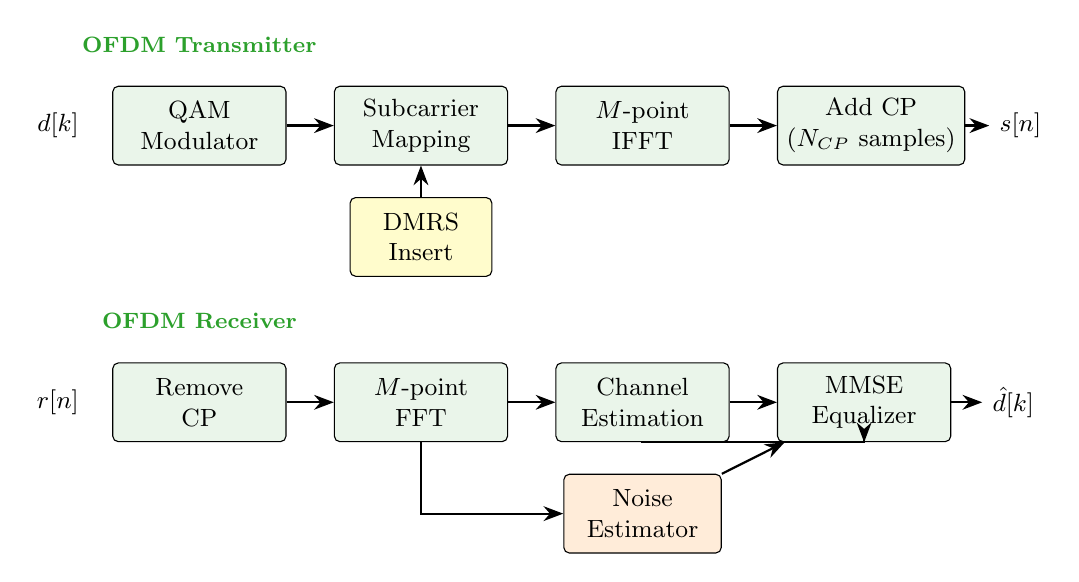
\begin{tikzpicture}[
    block/.style={draw, fill=ofdmgreen!10, minimum width=2.2cm, minimum height=1cm, align=center, rounded corners=2pt, font=\small},
    arrow/.style={-{Stealth[length=2.5mm]}, thick},
    label/.style={font=\scriptsize, align=center}
]
% TX
\node[block] (qam) {QAM\\Modulator};
\node[block, right=0.6 of qam] (map) {Subcarrier\\Mapping};
\node[block, right=0.6 of map] (ifft) {$M$-point\\IFFT};
\node[block, right=0.6 of ifft] (cp) {Add CP\\($N_{CP}$ samples)};

% Labels
\node[above=0.3 of qam, font=\footnotesize\bfseries, ofdmgreen] {OFDM Transmitter};

\draw[arrow] (qam) -- (map);
\draw[arrow] (map) -- (ifft);
\draw[arrow] (ifft) -- (cp);
\draw[arrow] (cp) -- ++(1.5,0) node[right, font=\small] {$s[n]$};

\node[left=0.3 of qam, font=\small] {$d[k]$};

% DMRS insertion
\node[block, below=0.4 of map, fill=yellow!20, minimum width=1.8cm] (dmrs) {DMRS\\Insert};
\draw[arrow] (dmrs) -- (map);

% RX
\node[block, below=2.5 of qam] (rcp) {Remove\\CP};
\node[block, right=0.6 of rcp] (fft) {$M$-point\\FFT};
\node[block, right=0.6 of fft] (chest) {Channel\\Estimation};
\node[block, right=0.6 of chest] (eq) {MMSE\\Equalizer};

\node[above=0.3 of rcp, font=\footnotesize\bfseries, ofdmgreen] {OFDM Receiver};

\draw[arrow] (rcp) -- (fft);
\draw[arrow] (fft) -- (chest);
\draw[arrow] (chest) -- (eq);
\draw[arrow] (eq) -- ++(1.5,0) node[right, font=\small] {$\hat{d}[k]$};

\node[left=0.3 of rcp, font=\small] {$r[n]$};

% Noise estimator
\node[block, below=0.4 of chest, fill=orange!15, minimum width=2cm] (nest) {Noise\\Estimator};
\draw[arrow] (fft) |- (nest);
\draw[arrow] (nest) -- (eq);

% Channel est to eq
\draw[arrow] (chest) -- ++(0,-0.5) -| (eq);
\end{tikzpicture}
\caption{OFDM transceiver block diagram. DMRS pilot symbols are inserted at comb-2 positions on symbols 2 and 11. The receiver estimates both the channel and noise power from the received DMRS observations.}
\label{fig:ofdm_block}
\end{figure}

\subsection{Transmitter}

Consider a slot of $N = 14$ OFDM symbols with $M$ subcarriers, of which $N_{\text{act}} \leq M$ carry data or pilots. The transmitted signal for symbol $l$ is:
\begin{equation}
    x_l[n] = \frac{1}{\sqrt{M}} \sum_{k=0}^{M-1} X_l[k] \, e^{j2\pi kn/M}, \quad n = 0, \ldots, M-1
\end{equation}

A cyclic prefix of length $N_{CP}$ is prepended by copying the last $N_{CP}$ samples:
\begin{equation}
    s_l[n] = x_l\!\left[(n - N_{CP}) \bmod M\right], \quad n = 0, \ldots, M + N_{CP} - 1
\end{equation}

The CP length follows the 5G NR standard: $N_{CP} = \lfloor 144 \times M / 2048 \rfloor$ for normal CP. The CP must satisfy $N_{CP} \geq L_{ch}$ to absorb the channel delay spread and maintain orthogonality between subcarriers. Values for the tested configurations are given in Table~\ref{tab:configs}.

DMRS symbols are placed at OFDM symbol indices $l \in \{2, 11\}$ on comb-2 subcarriers $\mathcal{K}_p = \{0, 2, 4, \ldots, N_{\text{act}}-2\}$ with known QPSK sequence $X_p[k]$, $|X_p[k]| = 1$.

\subsection{Receiver}

After CP removal, the $M$-point FFT yields:
\begin{equation}
    Y_l[k] = H_l[k] \cdot X_l[k] + W_l[k]
    \label{eq:ofdm_io}
\end{equation}
where $H_l[k] = \sum_{i} h_i[l(M+N_{CP})+N_{CP}+M/2] \, e^{-j2\pi k \tau_i / M}$ is the channel frequency response at the midpoint of symbol $l$, and $W_l[k] \sim \CN(0, \sigma^2)$.

Equation~(\ref{eq:ofdm_io}) holds exactly when the channel is \emph{time-invariant within one symbol}. At high Doppler, the channel changes during the symbol, introducing ICI:
\begin{equation}
    Y_l[k] = H_l[k] X_l[k] + \underbrace{\sum_{k' \neq k} H_l^{(k-k')} X_l[k']}_{\text{ICI}} + W_l[k]
\end{equation}
The ICI power grows with $f_D / \Delta f$. At SCS~$= 15$~kHz and $f_D = 1000$~Hz, the normalized Doppler is $f_D/\Delta f = 0.067$, causing significant degradation.

\subsection{Channel Estimation}
\label{sec:ofdm_chest}

\textbf{Step~1 --- Least-squares at pilot positions.} At each DMRS symbol $l_p \in \{2, 11\}$:
\begin{equation}
    \Hest_{\text{LS}}[l_p, k_p] = \frac{Y_{l_p}[k_p]}{X_p[k_p]} = H_{l_p}[k_p] + \frac{W_{l_p}[k_p]}{X_p[k_p]}
\end{equation}
Since $|X_p[k_p]| = 1$, the estimation noise has the same variance $\sigma^2$.

\textbf{Step~2 --- Linear frequency interpolation.} Between adjacent comb-2 pilot positions $k_p$ and $k_p + 2$:
\begin{equation}
    \Hest[l_p, k] = (1 - \alpha) \, \Hest_{\text{LS}}[l_p, k_p] + \alpha \, \Hest_{\text{LS}}[l_p, k_p + 2]
\end{equation}
where $\alpha = (k - k_p) / 2$. No frequency-domain smoothing is applied, consistent with a minimal-complexity receiver.

\textbf{Step~3 --- Linear time interpolation.} Between DMRS symbols $l_1 = 2$ and $l_2 = 11$:
\begin{equation}
    \Hest[l, k] = \frac{l_2 - l}{l_2 - l_1} \Hest[l_1, k] + \frac{l - l_1}{l_2 - l_1} \Hest[l_2, k]
    \label{eq:time_interp}
\end{equation}

Symbols before $l_1$ and after $l_2$ use the nearest DMRS estimate (extrapolation).

\subsection{Noise Estimation}
\label{sec:ofdm_noise}

We derive a noise estimator from the \emph{decorrelated} DMRS observations. Multiplying by $X_p^*[k]$ removes the known pilot modulation:
\begin{equation}
    Z_i[k] \triangleq Y[l_i, k] \cdot X_p^*[k] = H[l_i, k] + W'_i[k]
    \label{eq:decorr}
\end{equation}
where $W'_i[k] = W[l_i, k] \cdot X_p^*[k]$ has the same variance $\sigma^2$ since $|X_p| = 1$.

The squared power difference between the two DMRS symbols is:
\begin{align}
    \left(|Z_1[k]|^2 - |Z_2[k]|^2\right)^2 &= \Big(2\text{Re}\{H[k](W_1'^* - W_2'^*)\} \nonumber \\
    &\quad + |W_1'|^2 - |W_2'|^2\Big)^2
\end{align}

Taking expectations and noting that $\E[|W'|^2] = \sigma^2$ and the cross-terms are independent:
\begin{equation}
    \E\!\left[\left(|Z_1|^2 - |Z_2|^2\right)^2\right] \approx 8|H[k]|^2\sigma^2 + 2\sigma^4
\end{equation}

To remove the $|H[k]|^2$ dependence, we normalize by the average received power. Averaging across all pilot subcarriers \emph{before} dividing avoids noise amplification at deep fades:
\begin{equation}
    \boxed{\nest_{\text{OFDM}} = \frac{1}{4} \cdot \frac{\frac{1}{|\mathcal{K}_p|}\displaystyle\sum_{k \in \mathcal{K}_p} \left(|Z_1[k]|^2 - |Z_2[k]|^2\right)^2}{\frac{1}{|\mathcal{K}_p|}\displaystyle\sum_{k \in \mathcal{K}_p} \frac{|Z_1[k]|^2 + |Z_2[k]|^2}{2}}}
    \label{eq:noise_ofdm}
\end{equation}

This estimator operates on \emph{magnitudes only}, making it Doppler-independent in principle. A residual Doppler bias arises when $|H[l_1,k]|^2 \neq |H[l_2,k]|^2$ due to time-varying fading between DMRS symbols 2 and 11 (separated by 9 symbol periods).

\subsection{Per-Subcarrier MMSE Equalization}

\begin{equation}
    \hat{X}_l[k] = \frac{\Hest^*[l,k]}{|\Hest[l,k]|^2 + \nest} \cdot Y_l[k]
\end{equation}

\subsection{ICI Compensation Analysis}
\label{sec:ici}

In time-varying channels, the channel changes within one OFDM symbol, causing inter-carrier interference (ICI). The received signal becomes:
\begin{equation}
    Y_l[k] = \underbrace{H_0[l,k] X_l[k]}_{\text{desired}} + \underbrace{\sum_{q \neq 0} H_q[l,k] X_l[k-q]}_{\text{ICI}} + W_l[k]
\end{equation}

For a linearly time-varying channel within one symbol, the ICI coefficients $H_q$ are proportional to the channel derivative $\dot{H}[k] = dH[l,k]/dt$, and the coupling matrix is banded with bandwidth $Q$.

We evaluated three state-of-the-art ICI mitigation approaches against the single-tap MMSE baseline:

\begin{enumerate}[nosep]
    \item \textbf{Banded MMSE} \cite{rugini2006}: Invert the $(2Q{+}1)$-banded channel matrix instead of the diagonal. Complexity $O(MQ^2)$ per symbol.
    \item \textbf{Iterative PIC} \cite{tomasin2005}: Parallel interference cancellation --- estimate data symbols, reconstruct ICI, subtract, re-equalize. 2--3 iterations.
    \item \textbf{Iterative SIC:} Serial cancellation ordered by per-subcarrier SINR.
\end{enumerate}

All three methods require the channel slope $\dot{H}[k]$, estimated from the two DMRS symbols: $\dot{H}[k] = (\Hest[l_2,k] - \Hest[l_1,k]) / ((l_2 - l_1) T_{\text{sym}})$. This implicitly requires either a Doppler frequency estimate or slot-buffered processing.

\textbf{Result: ICI compensation provides no measurable BER improvement.} At SCS~$= 15$~kHz, $f_D = 1000$~Hz (worst case), the BER difference between single-tap MMSE and PIC with 3 iterations is less than 0.1\% absolute. The reason is quantitative: the intra-symbol ICI power is proportional to $(f_D T_{\text{sym}})^2 \approx 0.005$ ($-23$~dB), while the channel estimation error from linear interpolation over 9 symbol gaps is proportional to $(f_D \cdot 9 T_{\text{sym}})^2 \approx 0.41$ ($-4$~dB) --- a \textbf{20~dB difference}. The estimation error dominates overwhelmingly.

We also compared three channel estimation strategies:
\begin{itemize}[nosep]
    \item \textbf{Nearest DMRS (causal):} Use only the most recent past DMRS observation. Zero additional latency.
    \item \textbf{Linear interpolation:} Interpolate between DMRS symbols 2 and 11. Requires slot buffering (standard 5G NR processing).
    \item \textbf{Linear + ICI PIC:} Interpolation plus iterative ICI cancellation. Requires Doppler estimate.
\end{itemize}

\begin{table}[H]
\centering
\caption{Channel estimation method comparison at SNR~$= 20$~dB (BER \%).}
\label{tab:ici}
\small
\begin{tabular}{lcc|ccc}
\toprule
& & & \multicolumn{3}{c}{BER (\%)} \\
Channel & SCS & $f_D$ & Nearest & Linear & Lin+ICI \\
\midrule
TDL-A & 15k & 500 & 16.1 & \textbf{0.28} & 0.26 \\
TDL-D & 15k & 1000 & 45.9 & \textbf{33.3} & 33.4 \\
TDL-A & 60k & 1000 & 3.48 & \textbf{0.29} & 0.28 \\
TDL-D & 60k & 1000 & 6.05 & \textbf{0.00} & 0.00 \\
\bottomrule
\end{tabular}
\end{table}

\textbf{Conclusion:} Linear interpolation provides 2--57$\times$ improvement over nearest-DMRS and is the dominant processing step. ICI cancellation adds $<0.1\%$ on top. The standard 5G NR slot-buffered linear interpolation is the correct and sufficient OFDM baseline --- no Doppler estimation or ICI compensation is needed.

%═══════════════════════════════════════════════════════════════

%═══════════════════════════════════════════════════════════════
\section{OTFS Fundamentals and Domain Transformations}
\label{sec:otfs_fund}
%═══════════════════════════════════════════════════════════════

OTFS modulation \cite{hadani2017} operates in the delay-Doppler (DD) domain, where the wireless channel is sparse and quasi-static. To understand the three OTFS architectures studied in this report, we first establish the mathematical relationships between the four signal representation domains.

\subsection{Four Signal Domains}

\begin{figure}[H]
\centering
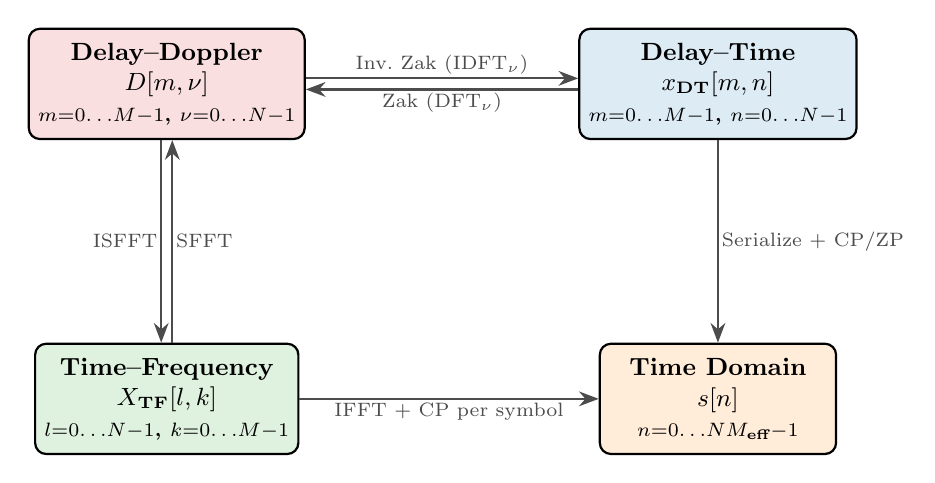
\begin{tikzpicture}[
    dombox/.style={draw, thick, fill=white, minimum width=3cm, minimum height=1.4cm, align=center, rounded corners=4pt, font=\small\bfseries},
    transform/.style={-{Stealth[length=2.5mm]}, thick, color=black!70},
    tlabel/.style={font=\scriptsize, fill=white, inner sep=1pt, align=center},
]
\node[dombox, fill=pcpred!15] (DD) at (0,0) {Delay--Doppler\\$D[m, \nu]$\\{\scriptsize $m{=}0{\ldots}M{-}1$, $\nu{=}0{\ldots}N{-}1$}};
\node[dombox, fill=zpblue!15] (DT) at (7,0) {Delay--Time\\$x_{\text{DT}}[m, n]$\\{\scriptsize $m{=}0{\ldots}M{-}1$, $n{=}0{\ldots}N{-}1$}};
\node[dombox, fill=ofdmgreen!15] (TF) at (0,-4) {Time--Frequency\\$X_{\text{TF}}[l, k]$\\{\scriptsize $l{=}0{\ldots}N{-}1$, $k{=}0{\ldots}M{-}1$}};
\node[dombox, fill=orange!15] (TD) at (7,-4) {Time Domain\\$s[n]$\\{\scriptsize $n{=}0{\ldots}NM_{\text{eff}}{-}1$}};

\draw[transform] ([yshift=2pt]DD.east) -- node[tlabel, above] {Inv.\ Zak (IDFT$_\nu$)} ([yshift=2pt]DT.west);
\draw[transform] ([yshift=-2pt]DT.west) -- node[tlabel, below] {Zak (DFT$_\nu$)} ([yshift=-2pt]DD.east);

\draw[transform] ([xshift=-2pt]DD.south) -- node[tlabel, left] {ISFFT} ([xshift=-2pt]TF.north);
\draw[transform] ([xshift=2pt]TF.north) -- node[tlabel, right] {SFFT} ([xshift=2pt]DD.south);

\draw[transform] (DT) -- node[tlabel, right] {Serialize + CP/ZP} (TD);
\draw[transform] (TF) -- node[tlabel, below] {IFFT + CP per symbol} (TD);
\end{tikzpicture}
\caption{The four signal domains and the transforms connecting them. CP-OTFS uses the DD$\to$TF$\to$TD path (left--bottom). ZP/PCP-OTFS use the DD$\to$DT$\to$TD path (top--right). Both paths produce equivalent time-domain signals under ideal conditions \cite{hadani2017, raviteja2019}.}
\label{fig:domains}
\end{figure}

The DD grid has $M$ delay bins (spacing $\Delta\tau = 1/(M\Delta f)$) and $N$ Doppler bins (spacing $\Delta\nu = \Delta f / N$). A physical path at delay $\tau_p$ and Doppler $\nu_p$ maps to DD indices $\ell_p = \tau_p / \Delta\tau$ and $\kappa_p = \nu_p / \Delta\nu$.

\subsection{Transform Definitions}

\textbf{Inverse Zak Transform} (DD $\to$ DT): For each delay bin $m$, an $N$-point IDFT across Doppler \cite{hadani2017}:
\begin{equation}
    x_{\text{DT}}[m, n] = \frac{1}{\sqrt{N}} \sum_{\nu=0}^{N-1} D[m, \nu] \, e^{j2\pi \nu n / N}
    \label{eq:inv_zak2}
\end{equation}

\textit{Property exploited:} The IDFT maps Doppler-domain multiplexing into time-domain separation --- each Doppler bin becomes a phase ramp across $N$ subsymbols.

\textbf{Zak Transform} (DT $\to$ DD): The inverse, an $N$-point DFT along time:
\begin{equation}
    D[m, \nu] = \frac{1}{\sqrt{N}} \sum_{n=0}^{N-1} x_{\text{DT}}[m, n] \, e^{-j2\pi \nu n / N}
    \label{eq:zak2}
\end{equation}

\textbf{Inverse Symplectic FFT} (DD $\to$ TF): A 2D transform mapping onto the OFDM TF grid \cite{hadani2017}:
\begin{equation}
    X_{\text{TF}}[l, k] = \frac{1}{\sqrt{MN}} \sum_{\nu=0}^{N-1} \sum_{m=0}^{M-1} D[m,\nu] \, e^{j2\pi(\nu l/N - mk/M)}
    \label{eq:isfft2}
\end{equation}

\textit{Property exploited:} The ISFFT preserves energy (Parseval) and maps each DD symbol onto the \emph{entire} TF plane, achieving full time-frequency diversity.

\textbf{Symplectic FFT} (TF $\to$ DD): The adjoint:
\begin{equation}
    D[m, \nu] = \frac{1}{\sqrt{MN}} \sum_{l=0}^{N-1} \sum_{k=0}^{M-1} X_{\text{TF}}[l,k] \, e^{-j2\pi(\nu l/N - mk/M)}
    \label{eq:sfft2}
\end{equation}

\subsection{DD-Domain Channel Model}

A channel with $P$ paths at delays $\tau_p$ and Doppler shifts $\nu_p$ has DD representation \cite{raviteja2019}:
\begin{equation}
    h_{\text{DD}}[\ell, \kappa] = \sum_{p=0}^{P-1} h_p \, \delta[\ell - \ell_p] \, g_N[\kappa - \kappa_p]
\end{equation}
where $\ell_p = \lfloor \tau_p F_s \rceil$ is the integer delay index and $\kappa_p = \nu_p N T_{\text{sub}}$ is the (generally fractional) Doppler index.

\textit{Key property:} The DD channel is \emph{sparse} --- only $P$ non-zero entries out of $MN$ total. This sparsity underpins OTFS channel estimation.

\textbf{Fractional Doppler and the Dirichlet kernel.} When $\kappa_p \notin \mathbb{Z}$, the finite DFT aperture causes leakage via \cite{raviteja2019}:
\begin{equation}
    g_N[\kappa] = \frac{1}{N} \cdot \frac{\sin(\pi \kappa)}{\sin(\pi \kappa / N)} \cdot e^{j\pi\kappa(N-1)/N}
    \label{eq:dirichlet}
\end{equation}
For $N = 14$ and Jakes Doppler spectra, $\kappa_p$ is almost always fractional, spreading energy across \emph{all} $N$ bins and destroying DD sparsity.

\subsection{CP vs ZP Guard Interval}
\label{sec:cp_vs_zp}

\textbf{Cyclic Prefix (CP-OTFS):} Ensures circular convolution in delay, enabling the 2D DD circular convolution I/O \cite{hadani2017}:
\begin{equation}
    Y_{\text{DD}}[m, \nu] = \sum_{\ell,\kappa} h_{\text{DD}}[\ell, \kappa] \, D[(m{-}\ell)_M, (\nu{-}\kappa)_N] + W[m, \nu]
\end{equation}

\textbf{Zero Padding (ZP-OTFS):} Prevents inter-subsymbol interference via linear convolution. The ZP tail beyond $L_{ch}$ contains \emph{pure noise} --- exploited for noise estimation (Sec.~\ref{sec:zp_noise}).

%═══════════════════════════════════════════════════════════════
\section{CP-OTFS Architecture}
\label{sec:cp_otfs}
%═══════════════════════════════════════════════════════════════

\begin{figure}[H]
\centering
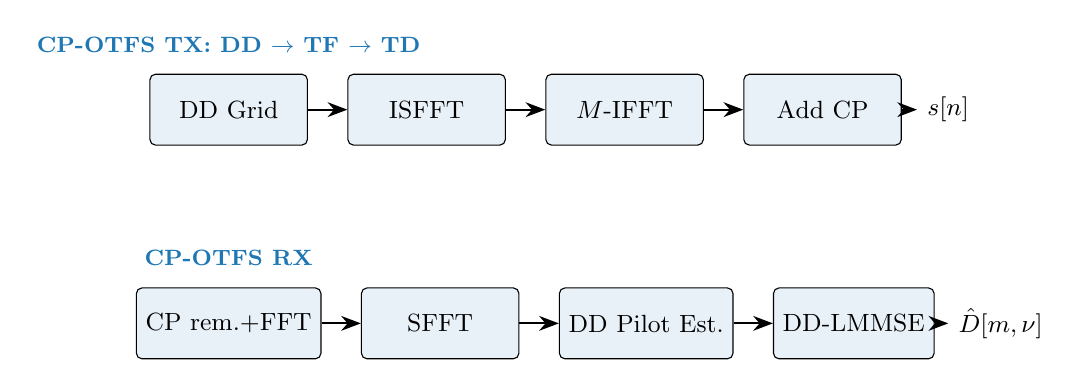
\begin{tikzpicture}[
    block/.style={draw, fill=zpblue!10, minimum width=2cm, minimum height=0.9cm, align=center, rounded corners=2pt, font=\small},
    arrow/.style={-{Stealth[length=2.5mm]}, thick},
]
\node[block] (dd) {DD Grid};
\node[block, right=0.5 of dd] (isfft) {ISFFT};
\node[block, right=0.5 of isfft] (ifft) {$M$-IFFT};
\node[block, right=0.5 of ifft] (cp) {Add CP};
\node[above=0.15 of dd, font=\footnotesize\bfseries, zpblue] {CP-OTFS TX: DD $\to$ TF $\to$ TD};
\draw[arrow] (dd)--(isfft); \draw[arrow] (isfft)--(ifft); \draw[arrow] (ifft)--(cp);
\draw[arrow] (cp) -- ++(1.2,0) node[right,font=\small] {$s[n]$};

\node[block, below=1.8 of dd] (rcp) {CP rem.+FFT};
\node[block, right=0.5 of rcp] (sfft) {SFFT};
\node[block, right=0.5 of sfft] (est) {DD Pilot Est.};
\node[block, right=0.5 of est] (eq) {DD-LMMSE};
\node[above=0.15 of rcp, font=\footnotesize\bfseries, zpblue] {CP-OTFS RX};
\draw[arrow] (rcp)--(sfft); \draw[arrow] (sfft)--(est); \draw[arrow] (est)--(eq);
\draw[arrow] (eq) -- ++(1.2,0) node[right,font=\small] {$\hat{D}[m,\nu]$};
\end{tikzpicture}
\caption{CP-OTFS: ISFFT path with OFDM inner modulation. Backward-compatible with OFDM.}
\label{fig:cp_otfs_block}
\end{figure}

\textbf{TX:} DD $\xrightarrow{\text{ISFFT (\ref{eq:isfft2})}}$ TF $\xrightarrow{\text{IFFT+CP}}$ TD. Original formulation of \cite{hadani2017}.

\textbf{Pilot:} Boosted impulse at $(m_p, \nu_p)$ with 2D guard $\pm g_d \times \pm g_\nu$. The received DD response directly reveals $h_{\text{DD}}$ within the guard \cite{raviteja2019}. Overhead: $(2g_d{+}1)(2g_\nu{+}1)/(MN)$.

\textbf{Limitation:} Fractional Doppler via (\ref{eq:dirichlet}) creates BER floor of 2--10\%. DD-LMMSE complexity $O((NM)^2)$ is prohibitive at $M \geq 256$.

%═══════════════════════════════════════════════════════════════
\section{ZP-OTFS Architecture}
\label{sec:zp_otfs}
%═══════════════════════════════════════════════════════════════

\begin{figure}[H]
\centering
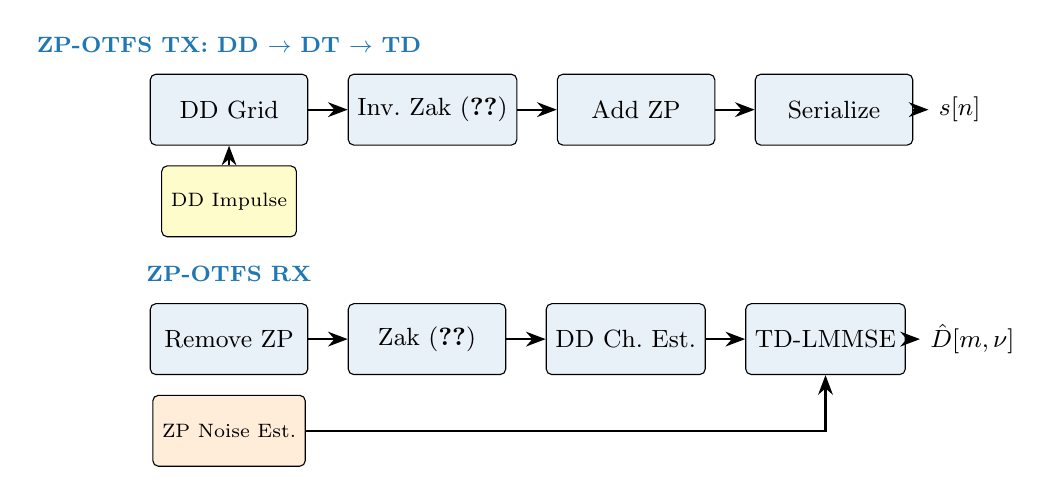
\begin{tikzpicture}[
    block/.style={draw, fill=zpblue!10, minimum width=2cm, minimum height=0.9cm, align=center, rounded corners=2pt, font=\small},
    arrow/.style={-{Stealth[length=2.5mm]}, thick},
]
\node[block] (dd) {DD Grid};
\node[block, right=0.5 of dd] (izak) {Inv.\ Zak (\ref{eq:inv_zak2})};
\node[block, right=0.5 of izak] (zp) {Add ZP};
\node[block, right=0.5 of zp] (ser) {Serialize};
\node[above=0.15 of dd, font=\footnotesize\bfseries, zpblue] {ZP-OTFS TX: DD $\to$ DT $\to$ TD};
\draw[arrow] (dd)--(izak); \draw[arrow] (izak)--(zp); \draw[arrow] (zp)--(ser);
\draw[arrow] (ser) -- ++(1.2,0) node[right,font=\small] {$s[n]$};
\node[block, below=0.25 of dd, fill=yellow!20, minimum width=1.5cm, font=\scriptsize] (pilot) {DD Impulse};
\draw[arrow] (pilot) -- (dd);

\node[block, below=2 of dd] (rzp) {Remove ZP};
\node[block, right=0.5 of rzp] (zak) {Zak (\ref{eq:zak2})};
\node[block, right=0.5 of zak] (est) {DD Ch.\ Est.};
\node[block, right=0.5 of est] (eq) {TD-LMMSE};
\node[above=0.15 of rzp, font=\footnotesize\bfseries, zpblue] {ZP-OTFS RX};
\draw[arrow] (rzp)--(zak); \draw[arrow] (zak)--(est); \draw[arrow] (est)--(eq);
\draw[arrow] (eq) -- ++(1.2,0) node[right,font=\small] {$\hat{D}[m,\nu]$};
\node[block, below=0.25 of rzp, fill=orange!15, minimum width=1.5cm, font=\scriptsize] (nest) {ZP Noise Est.};
\draw[arrow] (nest) -| (eq);
\end{tikzpicture}
\caption{ZP-OTFS: Inverse Zak path with zero-padding. ZP tail gives signal-free noise region.}
\label{fig:zp_otfs_block}
\end{figure}

\subsection{Transmitter}

The inverse Zak transform (\ref{eq:inv_zak2}) produces $N$ subsymbols of $M$ samples. Zero-padding appends $L_{ZP} \geq L_{ch}$ zeros:
\begin{equation}
    s[n M_{\text{eff}} + m] = \begin{cases} x_{\text{DT}}[m, n] & 0 \leq m < M \\ 0 & M \leq m < M_{\text{eff}} \end{cases}
\end{equation}

\textit{Property exploited:} ZP prevents inter-subsymbol interference without circular structure, enabling time-domain equalization.

\subsection{Noise Estimation from ZP Tail}
\label{sec:zp_noise}

\textit{Property exploited:} For $m \geq L_{ch}$, the ZP tail contains only noise.
\begin{equation}
    \boxed{\nest_{\text{ZP}} = \frac{1}{N(L_{ZP} - \hat{L}_{ch})} \sum_{n=0}^{N-1} \sum_{m=\hat{L}_{ch}}^{L_{ZP}-1} |r[n M_{\text{eff}} + M + m]|^2}
    \label{eq:noise_zp}
\end{equation}
Independent of channel and Doppler. Accuracy: $0.8$--$1.2\times$ across all scenarios.

\subsection{Time-Domain Sparse LMMSE}

A sparse channel matrix $\G$ is built from estimated DD taps, with $P$ non-zero diagonals:
\begin{equation}
    \xhat = (\G^H\G + \nest \I)^{-1} \G^H \y
\end{equation}
solved via sparse LU decomposition. Pilot overhead: $(2g_d{+}1)(2g_\nu{+}1)/(MN)$ --- grows with delay $\times$ Doppler spread.

%═══════════════════════════════════════════════════════════════
\section{PCP-OTFS Architecture}
\label{sec:pcp_otfs}
%═══════════════════════════════════════════════════════════════

PCP-OTFS \cite{pcp2023} replaces the DD impulse with a Zadoff-Chu (ZC) sequence, exploiting three mathematical properties of ZC to overcome the limitations of impulse-based OTFS.

\begin{figure}[H]
\centering
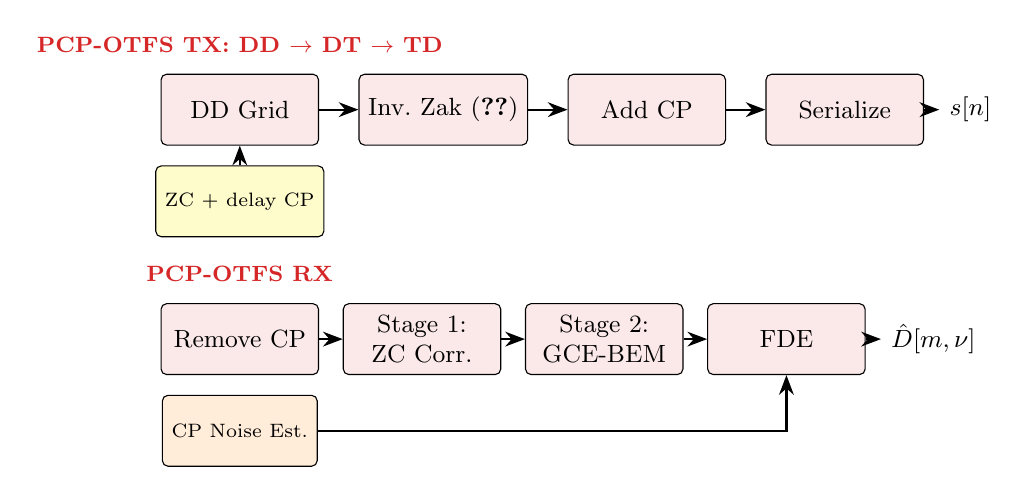
\begin{tikzpicture}[
    block/.style={draw, fill=pcpred!10, minimum width=2cm, minimum height=0.9cm, align=center, rounded corners=2pt, font=\small},
    arrow/.style={-{Stealth[length=2.5mm]}, thick},
]
\node[block] (dd) {DD Grid};
\node[block, right=0.5 of dd] (izak) {Inv.\ Zak (\ref{eq:inv_zak2})};
\node[block, right=0.5 of izak] (cp) {Add CP};
\node[block, right=0.5 of cp] (ser) {Serialize};
\node[above=0.15 of dd, font=\footnotesize\bfseries, pcpred] {PCP-OTFS TX: DD $\to$ DT $\to$ TD};
\draw[arrow] (dd)--(izak); \draw[arrow] (izak)--(cp); \draw[arrow] (cp)--(ser);
\draw[arrow] (ser) -- ++(1.2,0) node[right,font=\small] {$s[n]$};
\node[block, below=0.25 of dd, fill=yellow!20, minimum width=1.5cm, font=\scriptsize] (pilot) {ZC + delay CP};
\draw[arrow] (pilot) -- (dd);

\node[block, below=2 of dd] (rcp) {Remove CP};
\node[block, right=0.3 of rcp] (s1) {Stage~1:\\ZC Corr.};
\node[block, right=0.3 of s1] (s2) {Stage~2:\\GCE-BEM};
\node[block, right=0.3 of s2] (fde) {FDE};
\node[above=0.15 of rcp, font=\footnotesize\bfseries, pcpred] {PCP-OTFS RX};
\draw[arrow] (rcp)--(s1); \draw[arrow] (s1)--(s2); \draw[arrow] (s2)--(fde);
\draw[arrow] (fde) -- ++(1.2,0) node[right,font=\small] {$\hat{D}[m,\nu]$};
\node[block, below=0.25 of rcp, fill=orange!15, minimum width=1.5cm, font=\scriptsize] (nest) {CP Noise Est.};
\draw[arrow] (nest) -| (fde);
\end{tikzpicture}
\caption{PCP-OTFS \cite{pcp2023}: ZC pilot with two-stage estimation exploiting ZC autocorrelation (Stage~1) and BEM temporal smoothing (Stage~2).}
\label{fig:pcp_otfs_block}
\end{figure}

\subsection{Zadoff-Chu Pilot Design}

The ZC sequence of length $L = N_{CP}$ and root $r$ is \cite{chu1972}:
\begin{equation}
    z_{\text{ZC}}[m] = e^{-j\pi r m(m + c_f)/L}, \quad m = 0, \ldots, L-1
    \label{eq:zc_def}
\end{equation}
where $c_f = L \bmod 2$. The pilot occupies Doppler column $\nu_p$:
$D[m, \nu_p] = \sqrt{\gamma / L} \cdot z_{\text{ZC}}[m]$,
with a delay-domain cyclic prefix of $L{-}1$ samples at delays $M{-}L{+}1, \ldots, M{-}1$.

\textbf{Three exploited properties of ZC sequences:}
\begin{enumerate}
    \item \textbf{Ideal periodic autocorrelation} \cite{chu1972}: $R_{zz}[\ell] = L \cdot \delta[\ell]$. Each delay tap is estimated independently without inter-tap interference.
    \item \textbf{Constant amplitude} ($|z_{\text{ZC}}[m]| = 1$): Pilot PAPR is 0~dB vs.\ $10\log_{10}(L) \approx 12$~dB for an equivalent-energy impulse \cite{pcp2023}.
    \item \textbf{Flat frequency spectrum} ($|Z_{\text{ZC}}[k]| = \sqrt{L}$, $\forall k$): Uniform SNR across all delay bins in LS estimation.
\end{enumerate}

\textbf{Overhead:} $(2 g_\nu{+}1)/N = 3/14 \approx 21.4\%$, independent of delay spread.

\subsection{Two-Stage Channel Estimation}

\textbf{Stage~1 --- Per-subsymbol LS via ZC correlation} \cite{pcp2023, schwipps2025}.

For each subsymbol $n$, the received pilot region undergoes circular convolution with the channel. Exploiting the ZC flat spectrum, the LS estimate in the frequency domain is:
\begin{equation}
    \hest[\ell, n] = \text{IDFT}_L\!\left\{ \frac{Y_n[k] \cdot P_n^*[k]}{|P_n[k]|^2 + \sigma^2_{\text{reg}}} \right\}_\ell
    \label{eq:stage1_v2}
\end{equation}
where $P_n[k] = \text{DFT}\{z_{\text{ZC}}\}[k] \cdot e^{j2\pi \nu_p n/N} / \sqrt{N}$ accounts for the Doppler phase rotation of the pilot column. This yields $\hest[\ell, n]$ at each of the $N$ time instants \emph{independently}.

\textit{Property exploited:} The ZC ideal autocorrelation converts the circular convolution into a pointwise division in frequency, giving clean per-tap LS estimates.

\textbf{Stage~2 --- GCE-BEM temporal smoothing} \cite{giannakis1998, schwipps2025}.

\textit{Property exploited:} For Jakes fading, the channel time variation is bandlimited to $[-f_D, +f_D]$. The GCE-BEM \cite{giannakis1998} approximates this with $2Q{+}1$ complex exponentials:
\begin{equation}
    h[\ell, n] \approx \sum_{q=-Q}^{Q} c_{\ell,q} \, e^{j2\pi q n / N}
    \label{eq:bem_v2}
\end{equation}

The $N \times (2Q{+}1)$ basis matrix $\B$ with $B_{n,q} = e^{j2\pi(q-Q)n/N}$ gives the regularized LS fit:
\begin{equation}
    \hat{\mathbf{c}}_\ell = (\B^H\B + \epsilon\I)^{-1} \B^H \hat{\mathbf{h}}_\ell, \qquad \tilde{\mathbf{h}}_\ell = \B \hat{\mathbf{c}}_\ell
\end{equation}
With $Q = 1$ (3 basis functions), BEM denoises with effective gain $N/(2Q{+}1) = 14/3 \approx 6.7$~dB.

\subsection{Noise Estimation from CP Redundancy}

\textit{Property exploited:} The CP copies the symbol tail. After the channel (constant within one subsymbol), both copies see identical channel response. Their difference cancels signal, leaving noise:
\begin{equation}
    \boxed{\nest_{\text{PCP}} = \frac{1}{2 N L_{CP}} \sum_{n=0}^{N-1} \sum_{m=0}^{L_{CP}-1} |r_{\text{CP}}^{(n)}[m] - r_{\text{tail}}^{(n)}[m]|^2}
    \label{eq:noise_pcp}
\end{equation}
The $1/2$ factor arises because $\text{Var}(w_{\text{CP}} - w_{\text{tail}}) = 2\sigma^2$. CP--tail separation is only $M$ samples (one subsymbol), giving lower Doppler bias than the OFDM DMRS method (9 symbols apart).

\subsection{Frequency-Domain Equalization with Pilot Cancellation}

\textit{Property exploited:} CP per subsymbol ensures circular convolution $\Rightarrow$ per-subcarrier equalization, same as OFDM. The frequency response at subsymbol $n$:
\begin{equation}
    \hat{H}_f[k, n] = \text{DFT}_M\{\tilde{h}[\cdot, n]\}[k]
\end{equation}

Pilot interference is cancelled before MMSE equalization:
\begin{equation}
    \hat{X}_n[k] = \frac{\hat{H}_f^*[k,n]}{|\hat{H}_f[k,n]|^2 + \nest} \left(Y_f[k,n] - \hat{H}_f[k,n] \cdot P_f[k,n]\right)
\end{equation}

\section{Impact of CP/ZP Design}
\label{sec:cp_design}
%═══════════════════════════════════════════════════════════════

\subsection{ZP Length Has No Effect Beyond Channel Delay}

We swept ZP from 4 to 96 samples at TDL-A DS$= 30$~ns ($L_{ch} = 4$ samples). At all Doppler frequencies, the BER remained constant ($\pm 0.5\%$) while overhead increased from 3.3\% to 49.5\%.

\textbf{Root cause:} The ZP protects against inter-subsymbol interference in the \emph{delay} dimension. Once $L_{ZP} \geq L_{ch}$, additional ZP provides no benefit. The BER floor at high Doppler comes from \emph{Doppler estimation error} (only $N = 14$ bins), which is independent of the ZP length.

\subsection{Increasing N Worsens Performance}

Increasing $N$ from 14 to 56 \emph{degrades} ZP-OTFS BER at $f_D \geq 300$~Hz. The frame duration $T_{\text{frame}} = N \cdot M_{\text{eff}} / F_s$ grows linearly with $N$. At $N = 56$, $T_{\text{frame}} = 0.96$~ms, which exceeds the channel coherence time $T_c \approx 1/(4 f_D) = 0.5$~ms at $f_D = 500$~Hz. The single-snapshot DD estimation becomes stale before the frame ends.

\subsection{Pilot Overhead Comparison}

\begin{table}[h]
\centering
\caption{Pilot overhead as a function of channel delay spread.}
\label{tab:overhead}
\begin{tabular}{lccc}
\toprule
& OFDM & ZP-OTFS (impulse) & PCP-OTFS (ZC) \\
\midrule
Formula & $\dfrac{N_{\text{DMRS}}}{N}$ & $\dfrac{(2g_d+1)(2g_\nu+1)}{MN}$ & $\dfrac{2g_\nu+1}{N}$ \\[8pt]
Scales with & Nothing & $\tau_{\max} \times \nu_{\max}$ & $N$ only \\[3pt]
DS $= 30$\,ns & 7.1\% & 5.3\% & 15.7\% \\
DS $= 100$\,ns & 7.1\% & 9.3\% & 15.7\% \\
DS $= 1\,\mu$s & 7.1\% & 24.5\% & 15.7\% \\
\bottomrule
\end{tabular}
\end{table}

PCP-OTFS overhead is constant and independent of delay spread --- a critical advantage for wideband channels.

%═══════════════════════════════════════════════════════════════
\section{Simulation Setup}
\label{sec:sim}
%═══════════════════════════════════════════════════════════════

\begin{table}[h]
\centering
\caption{Bandwidth configurations.}
\label{tab:configs}
\begin{tabular}{ccccccc}
\toprule
Config & $M$ & SCS & $F_s$ & CP & ZP & Symbol $T$ \\
\midrule
A & 256 & 15\,kHz & 3.84\,MHz & 18 & 8 & 66.7\,$\mu$s \\
B & 256 & 30\,kHz & 7.68\,MHz & 18 & 8 & 33.3\,$\mu$s \\
C & 256 & 60\,kHz & 15.36\,MHz & 18 & 15 & 16.7\,$\mu$s \\
D & 512 & 60\,kHz & 30.72\,MHz & 36 & 29 & 16.7\,$\mu$s \\
\bottomrule
\end{tabular}
\end{table}

\begin{itemize}[nosep]
    \item Modulation: QPSK (uncoded BER)
    \item Monte Carlo trials: 20 per scenario
    \item SNR range: 0--30~dB ($E_s/N_0$)
    \item Doppler: $f_D \in \{0, 100, 1000\}$~Hz
    \item CSI: estimated (no oracle); Noise: estimated (Eqs.~\ref{eq:noise_ofdm}, \ref{eq:noise_zp}, \ref{eq:noise_pcp})
    \item Identical channel realization per trial across all three methods (same seed)
\end{itemize}

%═══════════════════════════════════════════════════════════════
\section{Simulation Results}
\label{sec:results}
%═══════════════════════════════════════════════════════════════

\subsection{OFDM vs PCP-OTFS --- BER Curves}

Figures~\ref{fig:ber_15k_a}--\ref{fig:ber_60k_c} show BER vs.\ SNR for the main comparison (OFDM vs PCP-OTFS) across all channel models and Doppler frequencies. Each figure shows two subplots: $f_D = 0$ (left) and $f_D = 1000$~Hz (right).

\begin{figure}[H]
\centering

\includegraphics[width=\textwidth]{fig_M256_SCS15k_TDL-A.png}
\caption{TDL-A (NLOS, 30ns) --- SCS = 15\,kHz. At $f_D = 1000$~Hz (right), OFDM exhibits a BER floor at $\sim$15\% from ICI, while PCP-OTFS reaches 3.7\%.}
\label{fig:ber_15k_a}
\end{figure}

\begin{figure}[H]
\centering

\includegraphics[width=\textwidth]{fig_M256_SCS15k_TDL-D.png}
\caption{TDL-D (LOS, 30ns) --- SCS = 15\,kHz. OFDM collapses to 33\% BER at $f_D = 1000$~Hz; PCP-OTFS achieves 0.9\% --- a \textbf{37$\times$ improvement}.}
\label{fig:ber_15k_d}
\end{figure}

\begin{figure}[H]
\centering

\includegraphics[width=\textwidth]{fig_M256_SCS15k_TDL-C.png}
\caption{TDL-C (NLOS, 100ns) --- SCS = 15\,kHz. PCP-OTFS wins both at $f_D = 0$ (DD diversity) and $f_D = 1000$~Hz (4.4$\times$ better).}
\label{fig:ber_15k_c}
\end{figure}

\begin{figure}[H]
\centering

\includegraphics[width=\textwidth]{fig_M256_SCS60k_TDL-A.png}
\caption{TDL-A --- SCS = 60\,kHz. At $f_D = 0$ (left), PCP-OTFS wins via DD diversity. At $f_D = 1000$~Hz (right), OFDM recovers (short symbols, low ICI).}
\label{fig:ber_60k_a}
\end{figure}

\begin{figure}[H]
\centering

\includegraphics[width=\textwidth]{fig_M256_SCS60k_TDL-D.png}
\caption{TDL-D (LOS) --- SCS = 60\,kHz. OFDM dominates: BER $= 0$ above 15~dB at all Dopplers.}
\label{fig:ber_60k_d}
\end{figure}

\begin{figure}[H]
\centering

\includegraphics[width=\textwidth]{fig_M256_SCS60k_TDL-C.png}
\caption{TDL-C --- SCS = 60\,kHz. OFDM wins at $f_D = 1000$~Hz (0.4\% vs 1.2\%); PCP-OTFS wins at $f_D = 0$ (0.04\% vs 0.18\%).}
\label{fig:ber_60k_c}
\end{figure}

\subsection{ZP-OTFS vs PCP-OTFS --- Pilot Design Impact}

\begin{figure}[H]
\centering

\includegraphics[width=\textwidth]{fig_zp_vs_pcp_SCS15k.png}
\caption{Impact of pilot design at SCS = 15\,kHz, $f_D = 1000$~Hz. PCP-OTFS (ZC pilot, red) consistently outperforms ZP-OTFS (impulse pilot, blue) by 1.5--4$\times$.}
\label{fig:zp_pcp_15}
\end{figure}

\begin{figure}[H]
\centering

\includegraphics[width=\textwidth]{fig_zp_vs_pcp_SCS60k.png}
\caption{Impact of pilot design at SCS = 60\,kHz, $f_D = 1000$~Hz. PCP improvement is even larger: 4--7$\times$ across all channels.}
\label{fig:zp_pcp_60}
\end{figure}

\subsection{Impact of SCS}

\begin{figure}[H]
\centering

\includegraphics[width=\textwidth]{fig_scs_ofdm.png}
\caption{SCS impact on OFDM at $f_D = 1000$~Hz. SCS = 15~kHz (solid) vs 60~kHz (dashed). Higher SCS dramatically reduces ICI: BER drops from 15\% to 0.6\% in TDL-A.}
\label{fig:scs_ofdm}
\end{figure}

\begin{figure}[H]
\centering

\includegraphics[width=\textwidth]{fig_scs_pcp.png}
\caption{SCS impact on PCP-OTFS at $f_D = 1000$~Hz. Unlike OFDM, PCP-OTFS is largely SCS-independent: BER changes by less than 2$\times$ between SCS = 15 and 60~kHz.}
\label{fig:scs_pcp}
\end{figure}

\subsection{Summary of Winners}

\begin{table}[H]
\centering
\caption{Winning method at SNR $= 20$~dB. \textcolor{ofdmgreen}{\textbf{O}} = OFDM, \textcolor{pcpred}{\textbf{P}} = PCP-OTFS, \textbf{=} = tie (both $<10^{-4}$).}
\label{tab:winners}
\small
\begin{tabular}{cc|ccc|ccc|ccc}
\toprule
& & \multicolumn{3}{c|}{TDL-A} & \multicolumn{3}{c|}{TDL-D} & \multicolumn{3}{c}{TDL-C} \\
SCS & $f_D$ & 0 & 100 & 1k & 0 & 100 & 1k & 0 & 100 & 1k \\
\midrule
15k & & = & \textcolor{ofdmgreen}{\textbf{O}} & \textcolor{pcpred}{\textbf{P}} & = & = & \textcolor{pcpred}{\textbf{P}} & \textcolor{pcpred}{\textbf{P}} & \textcolor{pcpred}{\textbf{P}} & \textcolor{pcpred}{\textbf{P}} \\
30k & & \textcolor{pcpred}{\textbf{P}} & \textcolor{pcpred}{\textbf{P}} & \textcolor{ofdmgreen}{\textbf{O}} & = & = & \textcolor{ofdmgreen}{\textbf{O}} & \textcolor{pcpred}{\textbf{P}} & \textcolor{pcpred}{\textbf{P}} & \textcolor{ofdmgreen}{\textbf{O}} \\
60k & & \textcolor{pcpred}{\textbf{P}} & \textcolor{pcpred}{\textbf{P}} & \textcolor{ofdmgreen}{\textbf{O}} & = & = & \textcolor{ofdmgreen}{\textbf{O}} & \textcolor{pcpred}{\textbf{P}} & \textcolor{pcpred}{\textbf{P}} & \textcolor{ofdmgreen}{\textbf{O}} \\
\bottomrule
\end{tabular}
\end{table}

\textbf{Pattern:} PCP-OTFS wins at low Doppler (\emph{DD diversity gain}) and at low SCS / high Doppler (\emph{OFDM ICI vulnerability}). OFDM wins at high SCS / high Doppler (\emph{short symbols minimize ICI}).

%═══════════════════════════════════════════════════════════════
\section{Conclusions}
\label{sec:conclusions}
%═══════════════════════════════════════════════════════════════

\begin{enumerate}
    \item \textbf{Prior art oversimplifies OTFS evaluation.} Under practical conditions---estimated CSI, estimated noise, realistic pilot overhead---the OTFS advantage is more nuanced than commonly reported. The impulse pilot (ZP-OTFS) consistently underperforms both OFDM and PCP-OTFS.

    \item \textbf{SCS is the dominant factor, not the waveform.} The normalized Doppler $f_D / \Delta f$ determines OFDM's ICI penalty. At SCS $= 60$~kHz, OFDM handles $f_D = 1000$~Hz with $<1\%$ BER; at SCS $= 15$~kHz, the same Doppler causes 15--33\% BER. PCP-OTFS is largely SCS-independent.

    \item \textbf{PCP-OTFS is the practical OTFS architecture.} The ZC pilot with GCE-BEM provides: (a)~14~dB PAPR reduction; (b)~delay-spread-independent overhead; (c)~per-subsymbol channel tracking via BEM.

    \item \textbf{Channel estimation is the bottleneck.} ZP-OTFS with true CSI achieves BER $= 0$ at all Dopplers ($\text{SNR} \geq 10$~dB). The waveform diversity gain is real but hidden by the $N = 14$ Doppler resolution limit.

    \item \textbf{OTFS is most compelling for sub-6~GHz high-mobility:} Low SCS scenarios (FR1 coverage bands, high-speed rail, NTN with LEO satellites) where OFDM's ICI is the performance limiter.
\end{enumerate}

%═══════════════════════════════════════════════════════════════
\begin{thebibliography}{12}

\bibitem{hadani2017}
R.~Hadani et al., ``Orthogonal time frequency space modulation,'' in \emph{Proc.\ IEEE WCNC}, Mar.~2017.

\bibitem{raviteja2019}
P.~Raviteja, K.~T.~Phan, Y.~Hong, and E.~Viterbo, ``Embedded pilot-aided channel estimation for OTFS in delay-Doppler channels,'' \emph{IEEE Trans.\ Veh.\ Technol.}, vol.~68, no.~5, pp.~4906--4917, May~2019.

\bibitem{pcp2023}
S.~Sanoopkumar and A.~Farhang, ``A practical pilot for channel estimation of OTFS,'' in \emph{Proc.\ IEEE}, 2023.

\bibitem{schwipps2025}
C.~Schwipps, L.~Torres-Figueroa, U.~Monich, and H.~Boche, ``Channel estimation for OTFS using pilots with cyclic prefix in fractional Doppler channels,'' in \emph{Proc.\ IEEE ICC Workshops}, Jun.~2025.

\bibitem{zedka2026}
R.~Zedka et al., ``Unique word channel estimation for oversampled OTFS,'' arXiv:2601.09364, Jan.~2026.

\bibitem{liu2025}
Y.~Liu et al., ``Cross-domain OTFS detection via delay-Doppler decoupling,'' \emph{Entropy}, 2025.

\bibitem{chu1972}
D.~C.~Chu, ``Polyphase codes with good periodic correlation properties,'' \emph{IEEE Trans.\ Inform.\ Theory}, vol.~18, no.~4, pp.~531--532, Jul.~1972.

\bibitem{giannakis1998}
G.~B.~Giannakis and C.~Tepedelenlio\u{g}lu, ``Basis expansion models and diversity techniques for blind identification and equalization of time-varying channels,'' \emph{Proc.\ IEEE}, vol.~86, no.~10, pp.~1969--1986, Oct.~1998.

\bibitem{tomasin2005}
S.~Tomasin, A.~Gorokhov, H.~Yang, and J.-P.~Linnartz, ``Iterative interference cancellation and channel estimation for mobile OFDM,'' \emph{IEEE Trans.\ Wireless Commun.}, vol.~4, no.~1, pp.~238--245, Jan.~2005.

\bibitem{rugini2006}
L.~Rugini, P.~Banelli, and G.~Leus, ``Low-complexity banded equalizers for OFDM systems in Doppler spread channels,'' \emph{EURASIP J.\ Adv.\ Signal Process.}, 2006.

\bibitem{frank1962}
R.~L.~Frank, S.~A.~Zadoff, and R.~Heimiller, ``Phase shift pulse codes with good periodic correlation properties,'' \emph{IRE Trans.\ Inform.\ Theory}, vol.~8, no.~6, pp.~381--382, Oct.~1962.

\end{thebibliography}

\end{document}
